\documentclass{article}

\usepackage[UTF8]{ctex}
\usepackage{amsmath}
%\usepackage{steinmetz}
\usepackage{graphicx}
\usepackage{geometry}
\geometry{a4paper,scale=0.75}
% left=2cm,right=2cm,top=1cm,bottom=1cm
\title{目标检测Notebook}
\author{叶亮}
\date{\today}
\begin{document} 
\maketitle
\section{Loss}
\subsection{IoU loss}
IoU Loss的基本计算公式为:
\begin{align}
\mathcal{L}_{IoU} = 1 - IoU
\end{align}
其中, IoU为预测和GT框的交并比,其他改进后的版本大多式在此基础上加入额外的惩罚项来有针对性地引导模型。其优点为:

1. 可以反映预测检测框与真实检测框的检测效果。

2. 尺度不变性,也就是对尺度不敏感(scale invariant), 在regression任务中,判断predict box和gt的距离最直接的指标就是IoU。(满足非负性;同一性;对称性;三角不等性)。

缺点:

1. 如果两个框没有相交,根据定义,IoU=0,不能反映两者的距离大小(重合度)。同时因为loss=0,没有梯度回传,无法进行学习训练。

2. IoU无法精确的反映两者的重合度大小。如下图所示,三种情况IoU都相等,但看得出来他们的重合度是不一样的,左边的图回归的效果最好,右边的最差。
\begin{figure}[htp]
\centering
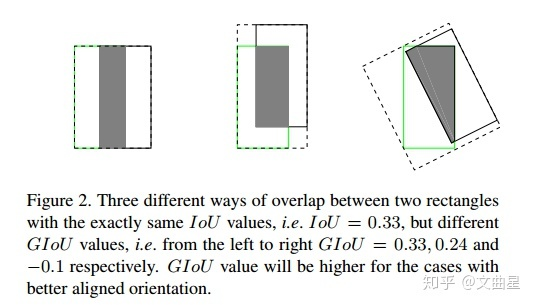
\includegraphics[scale=0.5]{images/IoU.jpg}
\caption{相同IoU的不同情况}
\label{Fig.IoU}
\end{figure}

\subsection{GIoU loss}
GIoU loss中的IoU部分替换成了GIoU,其计算方式如下:
\begin{align}
GIoU = IoU - \frac{\left| A_c - U \right|}{\left| A_c \right|}
\end{align}
其中,$A_c$表示两个框的最小闭包区域面积(同时包含预测和GT的最小框),然后计算闭包区域中不属于两个框的区域所占比重。特性:

1.与IoU相似,GIoU也是一种距离度量,作为损失函数的话, [公式] ,满足损失函数的基本要求;

2. GIoU对scale不敏感; 

3. GIoU是IoU的下界,在两个框无限重合的情况下,IoU=GIoU=1;

4. IoU取值[0,1],但GIoU有对称区间,取值范围[-1,1]。在两者重合的时候取最大值1,在两者无交集且无限远的时候取最小值-1,因此GIoU是一个非常好的距离度量指标。

5. 与IoU只关注重叠区域不同,GIoU不仅关注重叠区域,还关注其他的非重合区域,能更好的反映两者的重合度。
\subsection{DIoU loss}
DIoU要比GIou更加符合目标框回归的机制,将目标与anchor之间的距离,重叠率以及尺度都考虑进去,使得目标框回归变得更加稳定,不会像IoU和GIoU一样出现训练过程中发散等问题。
\begin{align}
DIoU = IoU - 	\frac{\rho^2(b,b^{gt})}{c^2}
\end{align}
其中,$\rho()$为欧式距离计算,$b$为中心点坐标,$c$为最小闭包的对角线长度:$c^2= cw^2+ch^2$.
Code optimization, the calculation of distance between two center points of bboxes.
$C$包含$x$和$y$,以下公式为$x$计算部分,$y$部分同理,最后求和.
\begin{equation}
\begin{aligned}
(C_1-C_2)^2)&= ((x1_{C1}+x2_{C1})/2-(x1_{C2}+x2_{C2})/2)^2 \\
&=((x1_{C1}+x2_{C1})-(x1_{C2}+x2_{C2}))^2/4 \\
\end{aligned}
\end{equation}
\begin{figure}[htp]
\centering
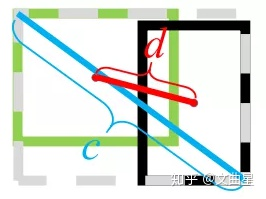
\includegraphics[scale=0.5]{images/DIoU.jpg}
\caption{DIoU:对anchor框和目标框之间的归一化距离进行了建模}
\label{Fig. DIoU}
\end{figure}
特性:

1. 与GIoU loss类似,DIoU loss($ \mathcal{L}_{DIoU}= 1- DIoU$)在与目标框不重叠时,仍然可以为边界框提供移动方向。

2. DIoU loss可以直接最小化两个目标框的距离,因此比GIoU loss收敛快得多。
3. 对于包含两个框在水平方向和垂直方向上这种情况,DIoU损失可以使回归非常快,而GIoU损失几乎退化为IoU损失。
4. DIoU还可以替换普通的IoU评价策略,应用于NMS中,使得NMS得到的结果更加合理和有效。

\subsection{CIoU loss}
论文考虑到bbox回归三要素中的长宽比还没被考虑到计算中,因此,进一步在DIoU的基础上提出了CIoU。其惩罚项如下面公式:
\begin{align}
\mathcal{R}_{CIoU} = \frac{\rho^2(b,b^{gt})}{c^2} + \alpha v
\end{align}
其中,$v$用来度量长宽比的相似性,定义为:$v=\frac{4}{\pi^2}(\arctan{\frac{w^{gt}}{h^{gt}}}- \arctan{\frac{w}{h}})^2 $, $\alpha$为权重函数,定义为:$\alpha = \frac{v}{(1-IoU)+v}$。最后,CIoU loss的梯度类似于DIoU loss,但还要考虑$v$的梯度。在长宽在 $[0,1]$ 的情况下,对$\arctan$进行求导时$w^2+h^2$的值通常很小,会导致梯度爆炸,因此在 $\frac{1}{w^2+h^2}$实现时将替换成1。在使用pytorch实现时,计算$\alpha$时使用 torch.no\_grad()来避免计算$\alpha$的损失,以此来保证合理的收敛过程。

\subsection{BIoU loss}

\section{Activation}
\subsection{Sigmoid}
Sigmoid函数,其公式如下:
\begin{align}
\sigma(x) = \frac{1}{1+e^{-x}} \\
\sigma'(x) = \sigma(x) \cdot (1 - \sigma(x))
\end{align}
\begin{figure}[htp]
\centering
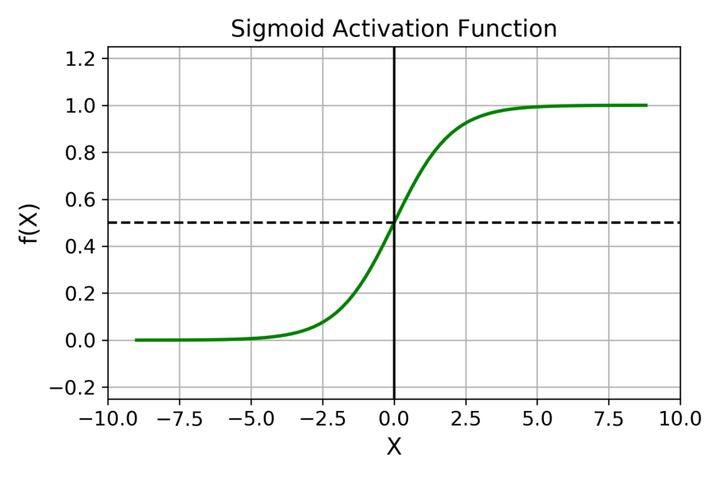
\includegraphics[scale=0.3]{images/activation/sigmoid.jpg}
\caption{Sigmoid函数}
\label{Fig.sigmoid}
\end{figure}
在什么情况下适合使用 Sigmoid激活函数呢?

1. Sigmoid 函数的输出范围是 0 到 1。由于输出值限定在 0 到 1,因此它对每个神经元的输出进行了归一化;

2. 用于将预测概率作为输出的模型。由于概率的取值范围是 0 到 1,因此 Sigmoid 函数非常合适;梯度平滑,避免「跳跃」的输出值;

3. 函数是可微的。这意味着可以找到任意两个点的 sigmoid 曲线的斜率;

4. 明确的预测,即非常接近 1 或 0。

Sigmoid激活函数有哪些缺点?

1. 倾向于梯度消失;

2. 函数输出不是以 0 为中心的,这会降低权重更新的效率;

3. Sigmoid 函数执行指数运算,计算机运行得较慢。

\subsection{Tanh}
双曲正切函数,其图形也是S形,公式如下:
\begin{align}
tanh(x) = \frac{2}{1+e^{-2x}} - 1 = \frac{\exp(x) - \exp(-x)} {\exp(x) + \exp(-x)}  \\
tanh'(x) = 1 - tanh^2(x)
\end{align}
\begin{figure}[htp]
\centering
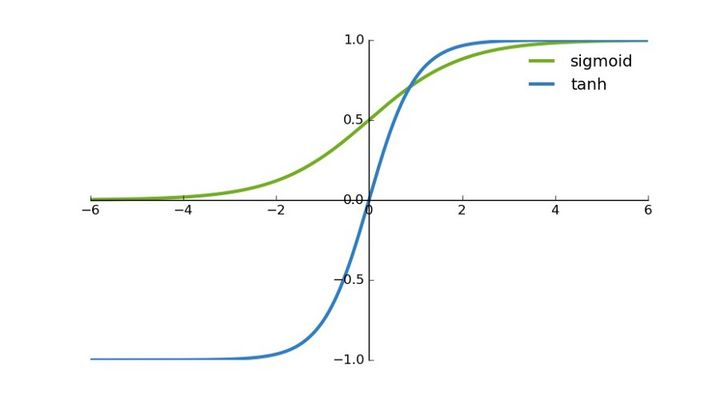
\includegraphics[scale=0.3]{images/activation/tanh.jpg}
\caption{Tanh函数}
\label{Fig.tanh}
\end{figure}
相比sigmoid, tanh的优势体现在:

首先,当输入较大或较小时,输出几乎是平滑的并且梯度较小,这不利于权重更新。二者的区别在于输出间隔,tanh 的输出间隔为 1,并且整个函数以 0 为中心,比 sigmoid 函数更好;

tanh函数的缺点同sigmoid函数的第一个缺点一样,当x很大或很小时,导数接近于 0 ,会导致梯度很小,权重更新非常缓慢,即梯度消失问题。

在一般的二元分类问题中,tanh 函数用于隐藏层,而 sigmoid 函数用于输出层.

\subsection{ReLU}
ReLU的公式如下:
\begin{equation}
relu(x) = \begin{cases}
	x,  x>=0 \\
	0, x < 0
\end{cases}
\end{equation}
\begin{figure}[htp]
\centering
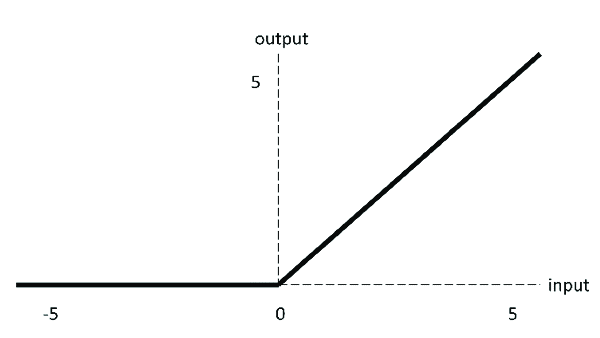
\includegraphics[scale=0.4]{images/activation/relu.png}
\caption{ReLU函数}
\label{Fig.relu}
\end{figure}

ReLU6的公式如下,这是为了在移动端设备 float16/int8 的低精度的时候也能有很好的数值分辨率:
\begin{align*}
\text{ReLU6}(x) = \min(\max(0,x), 6)
\end{align*}

优点:
输入为正时,不存在梯度饱和问题;计算速度快。

缺点:

Dead ReLU 问题。当输入为负时,ReLU 完全失效,在正向传播过程中,这不是问题。有些区域很敏感,有些则不敏感。但是在反向传播过程中,如果输入负数,则梯度将完全为零,sigmoid 函数和 tanh 函数也具有相同的问题;

输出为 0 或正数,这意味着 ReLU 函数不是以 0 为中心的函数。

\subsection{Leaky ReLU \& Parametric ReLU}
\begin{equation}
LReLU(x) = \begin{cases}
	x, x>0 \\
	ax, x<=0
	\end{cases}
\end{equation}
\begin{figure}[htp]
\centering
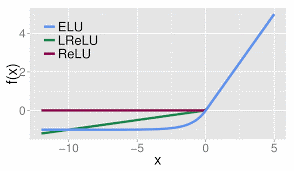
\includegraphics[scale=1]{images/activation/elu.png}
\caption{ReLU、Leaky ReLU、ELU}
\label{Fig.elu}
\end{figure}
特性:

Leaky ReLU 通过把 x 的非常小的线性分量给予负输入(0.01x)来调整负值的零梯度(zero gradients)问题;如果$a$是可以学习的参数,则为\textbf{PReLU}(Parametric ReLU).

leak 有助于扩大 ReLU 函数的范围,通常 a 的值为 0.01 左右;

Leaky ReLU 的函数范围是(负无穷到正无穷)。

\subsection{ELU}
ELU 的提出也解决了 ReLU 的问题。与 ReLU 相比,ELU 有负值,这会使激活的平均值接近零。均值激活接近于零可以使学习更快,因为它们使梯度更接近自然梯度。
\begin{equation}
        \text{ELU}(x) = \begin{cases}
        x, & \text{ if } x > 0\\
        \alpha * (\exp(x) - 1), & \text{ if } x \leq 0
        \end{cases}
\end{equation}

ELU 具有 ReLU 的所有优点,并且:

1. 没有 Dead ReLU 问题,输出的平均值接近 0,以 0 为中心;

2. ELU 通过减少偏置偏移的影响,使正常梯度更接近于单位自然梯度,从而使均值向零加速学习;

3. ELU 在较小的输入下会饱和至负值,从而减少前向传播的变异和信息。

一个小问题是它的计算强度更高。与 Leaky ReLU 类似,尽管理论上比 ReLU 要好,但目前在实践中没有充分的证据表明 ELU 总是比 ReLU 好。


\subsection{SiLU / Swish}
Sigmoid Linear Unit
\begin{align}
\text{silu}(x) = x * \sigma(x), \text{where } \sigma(x) \text{ is the logistic sigmoid.}
\end{align}
\begin{figure}[htp]
\centering
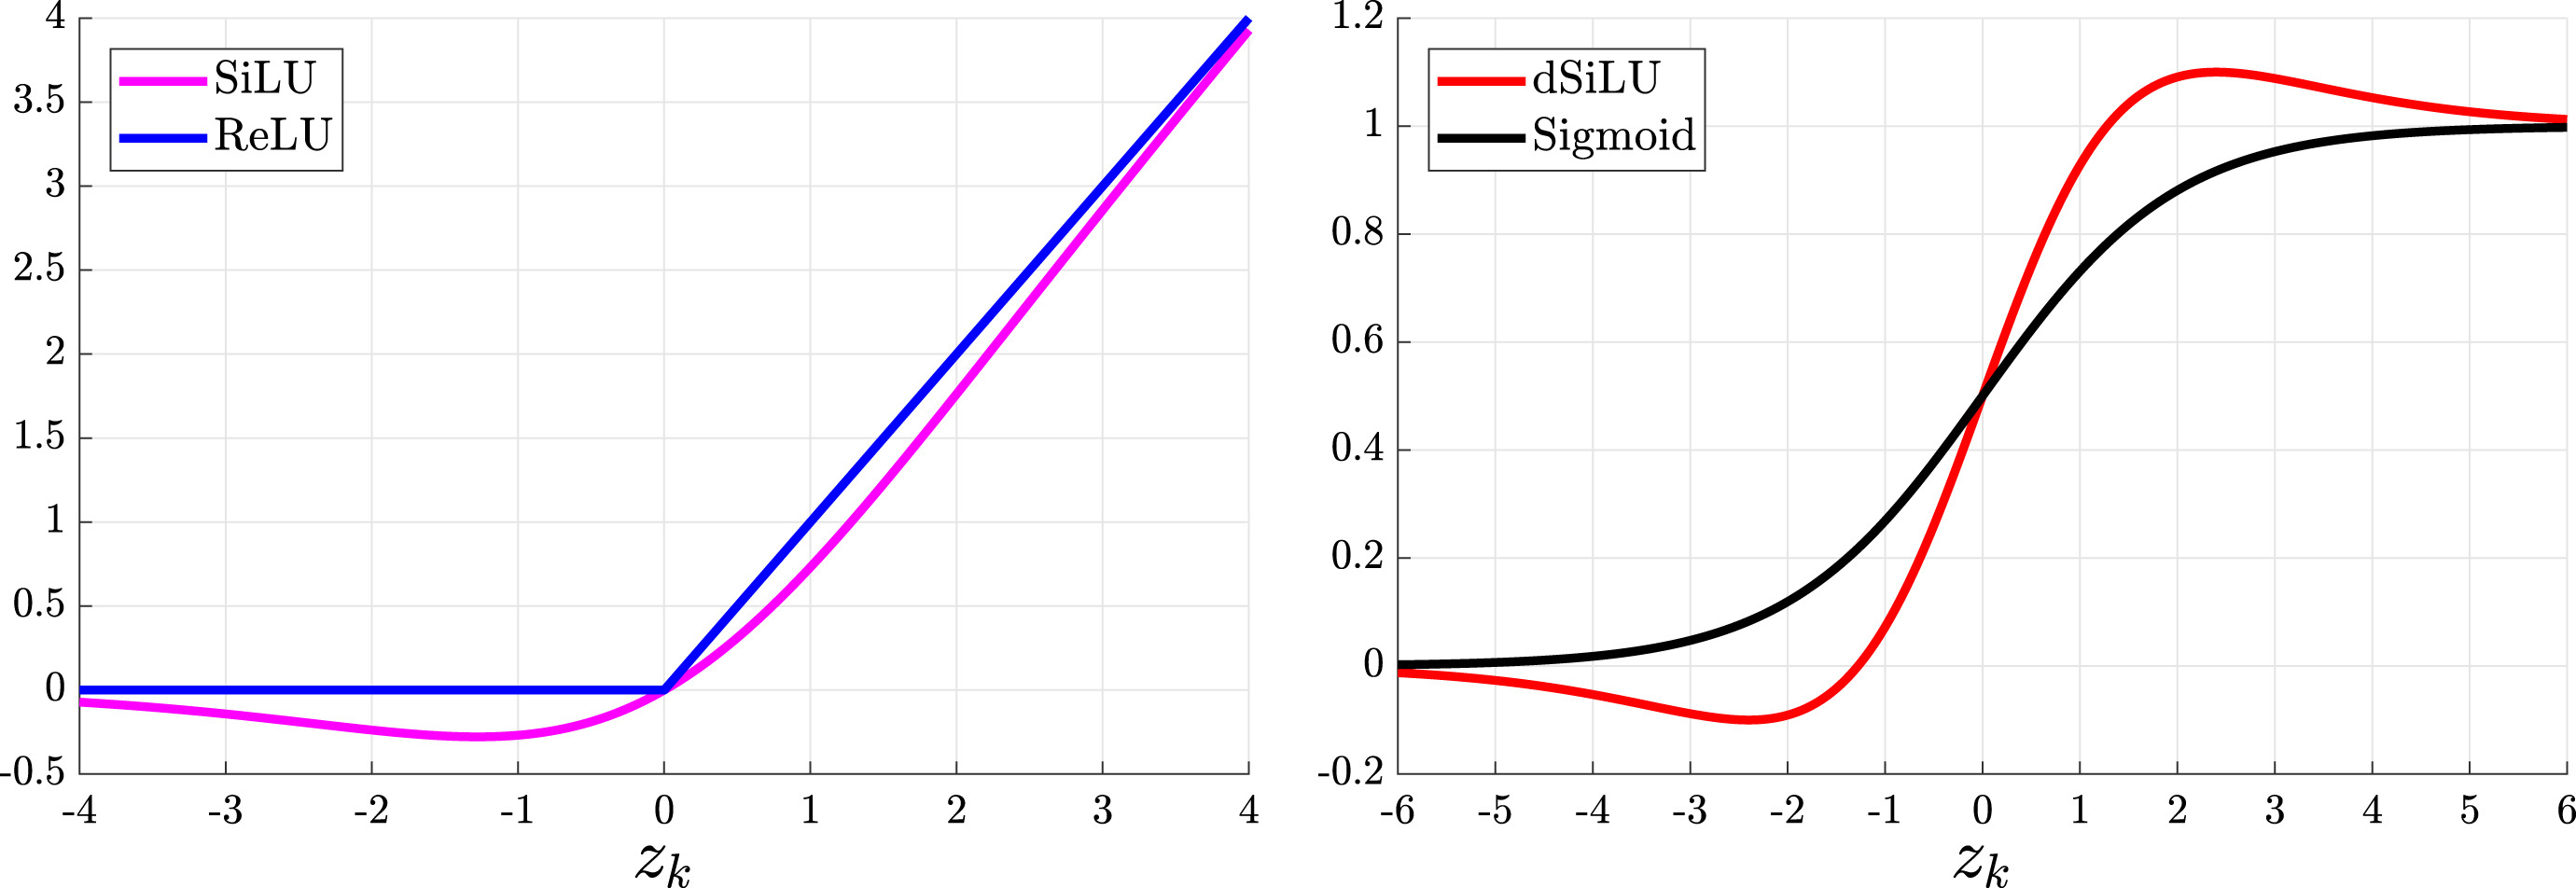
\includegraphics[scale=1]{images/activation/SiLU.jpg}
\caption{The activation functions of the SiLU and the ReLU (left panel), and the dSiLU and the sigmoid unit (right panel)}
\label{SiLU}
\end{figure}

Swish 的设计受到了 LSTM 和高速网络中 gating 的 sigmoid 函数使用的启发。使用相同的 gating 值来简化 gating 机制,这称为 self-gating。self-gating 的优点在于它只需要简单的标量输入,而普通的 gating 则需要多个标量输入。这使得诸如 Swish 之类的 self-gated激活函数能够轻松替换以单个标量为输入的激活函数(例如 ReLU),而无需更改隐藏容量或参数数量。
Swish激活函数的主要优点如下:

「无界性」有助于防止慢速训练期间,梯度逐渐接近 0 并导致饱和;(同时,有界性也是有优势的,因为有界激活函数可以具有很强的正则化,并且较大的负输入问题也能解决);
平滑度在优化和泛化中起了重要作用。

\subsection{Hard swish}
\begin{equation}
        \text{Hardswish}(x) = \begin{cases}
            0 & \text{if~} x \le -3, \\
            x & \text{if~} x \ge +3, \\
            x \cdot (x + 3) /6 & \text{otherwise}
        \end{cases}
\end{equation}
主要是解决移动端下精度较低时的计算问题。
\begin{figure}[htp]
\centering
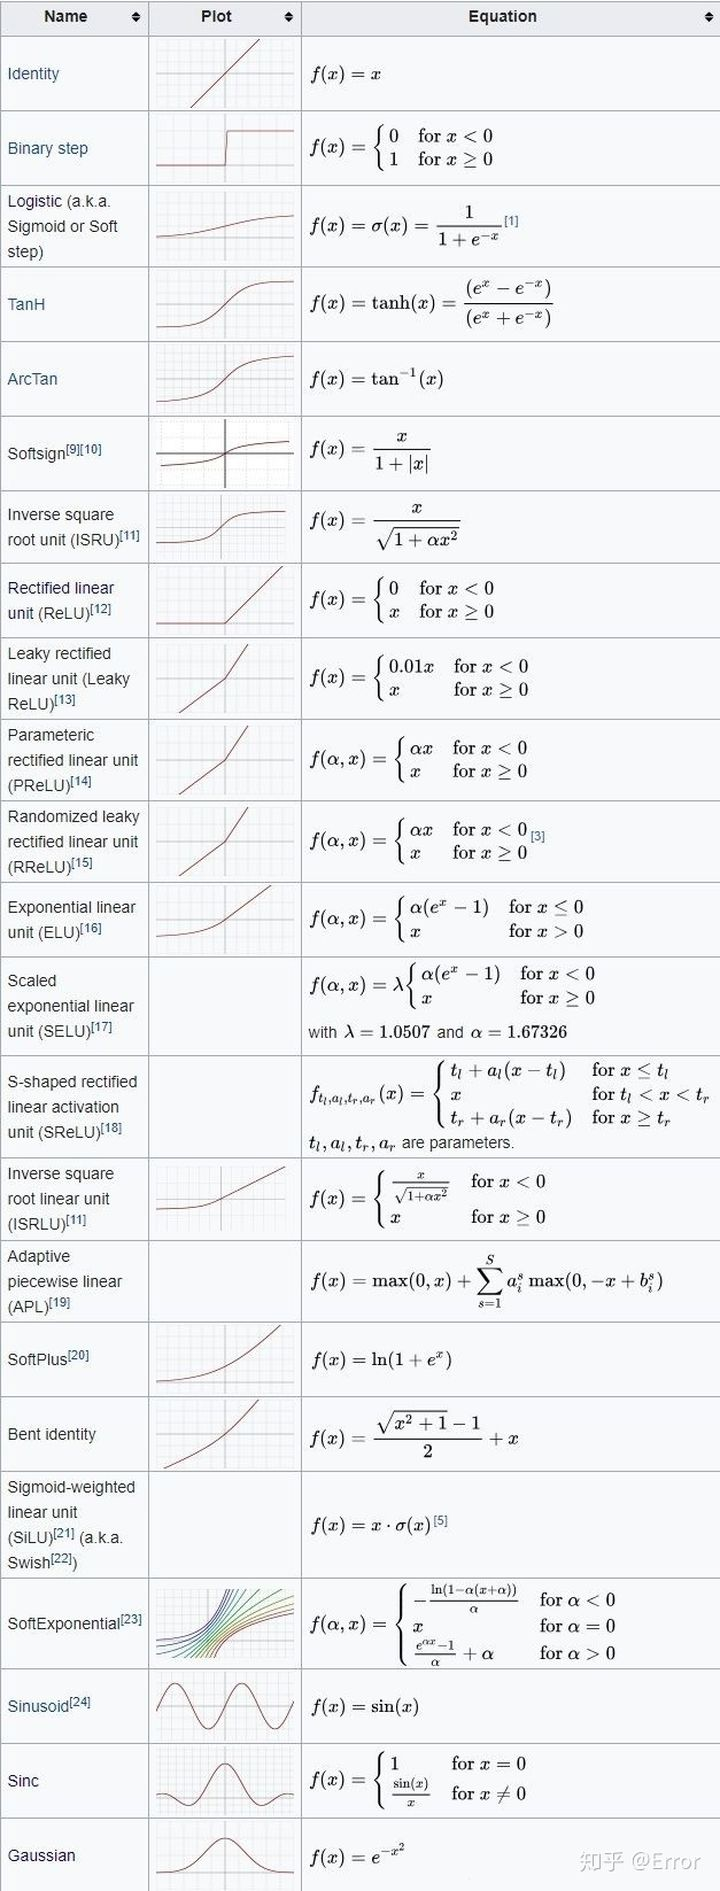
\includegraphics[scale=0.4]{images/activation/activation.jpg}
\caption{激活函数}
\end{figure}

\section{mmdetection}

\subsection{anchor}
mmdetection中,在retinanet, R-CNN等非ssd系列检测器的grid anchor生成中,在grid中每个anchor的坐标表示为(xmin,ymin,xmax,ymax)。anchor参数包含strides, ratios, scales, base sizes等. 其中strides为特征图的步长,ratios为宽高比,scales为anchor的缩放因子。计算过程如下:

1. 根据featmap生成grid.其中grid坐标为i * featmap size for i in grid size.

2. grid中每个cell根据 ratios,  scales和base sizes计算anchors,$xmin = grid_i -  basesize*scales*ratios, xmax = grid_i +basesize*scales*ratios$.
每个anchor的形式为(xmin,ymin,xmax,ymax),且均

 具体计算方式可参考\textbf{core/anchor/anchor\_generator.py}中部分。

\subsection{coder}
在RetinaNet、SSD、Cascade R-CNN等网络中,网络预测的bbox都会进行Delta xywh编码,即将原始的(xmin, ymin, xmax, ymax)进行编码,计算proposals相对GT的距离,得到(dx,dy,dw,dh),来减小回归的过拟合,提升回归的稳定性。其中编码后的x为中心点。
\begin{equation}
\begin{aligned}
&\delta_x = (g_x-p_x)/p_w	   & \delta_y = (g_y - p_y)/p_h \\
&\delta_w = \log{\frac{g_w}{p_w}}	&\delta_h = \log{\frac{g_h}{p_h}}
\end{aligned}\label{bbox_coder}
\end{equation}

上述公式计算得到的$\delta$值通常很小,因为网络通常只对p进行少量微调,导致回归loss比分类loss小很多。为了提升学习的有效性,$\delta$通常需要经过均值和方差进行标准化.

\begin{equation}
\begin{aligned}
\delta_{x}^{'}=\frac{\delta_x-\mu_x}{\rho_x}
\end{aligned}
\end{equation}

\subsection{two-stage}
mmdetection中的二阶段检测网络,首先使用RPN-FPN网络,得到多个level的特征图,然后使用多个level的特征图生成proposals,并使用NMS进行过滤。然后利用过滤后的proposals,在对应特征图上进行ROIAlign和ROIPool.在RPN阶段,计算loss时分类loss只计算class-agnostic loss,即采样到的gt targets为正的框。
\subsubsection{ROI Pool}
ROI pool根据生成的proposals,(xyxy),在对应的feature maps上进行裁剪,将对应坐标内的特征图分成$s*s$块状网格,每个网络里面可能由多个值,然后使用最大池化对每个网络内的多个值进行池化,得到$s*s$的尺寸输出。在对特征图进行分块时,ROI pool使用直接取整的方式,以一个$8*8$的特征图为例,输出$2*2$的池化后的特征图。假设(xyxy)为(0,3,7,8),则proposal的原始h,w为7,5.则1)5/2 = 2.5 --> 2, 剩下的为3,则2+3 向下取整floor; 2)7/2 = 3.5 -->3, 剩下的为4,则3+4
\begin{figure}
\centering
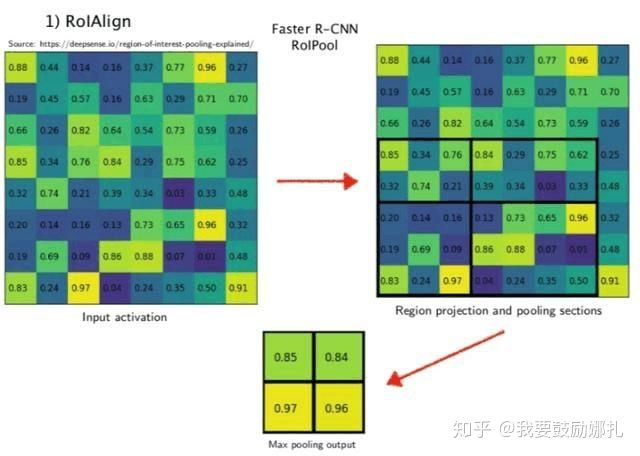
\includegraphics[scale=0.5]{images/roipool.jpg}
\caption{ROI-Pool过程}
\label{Fig.roi_pool}
\end{figure}

\section{training}
\subsection{Optimizer}
\subsubsection{warmup}
warmup通常有三个方式:linear, constant, exp. 通常需要设置warmup的迭代数$iter_{total}$和warmup的增加比率ratio,
\begin{align}
lr_t = lr_{constant}*ratio
\end{align}
\begin{equation}
\begin{aligned}
lr_t = lr_{const}*(1-k), \\
k= (1-iter_t /iter_{total}) * (1-ratio)
\end{aligned}
\end{equation}
\begin{align}
lr_t = lr_{const}*k, \\
k=ratio^{1-iter_t/iter_{total}}
\end{align}

\section{Yolov4}
Yolov4的实现过程中,anchor的生成以及label与anchor的对应关系的构建方法。如图\ref{Fig.yolo_bbox}.所示。
\subsection{Anchor generation \& target build}
与retinanet,rcnn系列等bbox预测不同的是,yolo模型推理得到的结果(x,y,w,h)需要经过如下公式进行编码:
\begin{equation}
\begin{aligned}
b_x = \sigma(t_x)+c_x \\
b_y = \sigma(t_y)+c_y \\
b_w = p_we^{t_w} \\
b_h = p_he^{t_h}
\end{aligned}
\end{equation}
\begin{figure}[htp!]
\centering
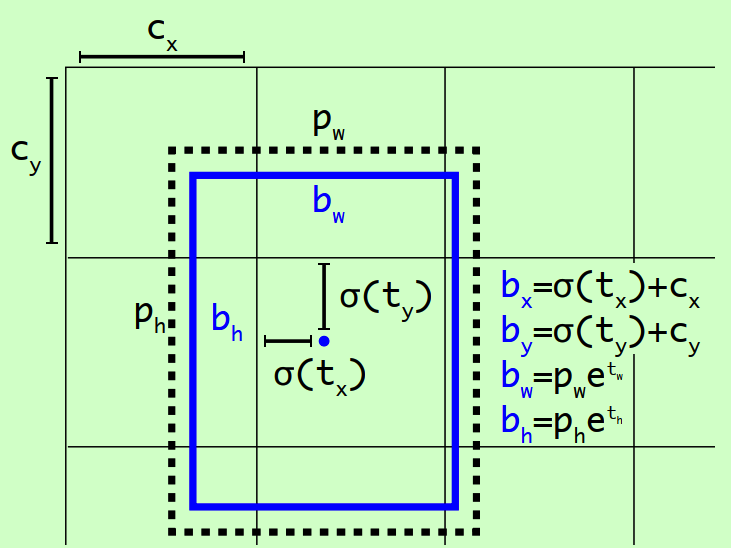
\includegraphics[scale=0.3]{images/yolo_bbox.png}
\caption{Yolo bbox prediction}
\label{Fig.yolo_bbox}
\end{figure}

\section{Yolov5}
\subsection{Model}
\textbf{Focus结构}: Focus模块中,首先将一幅图,按照隔点采样(::2,1::2)的方式,将一个图片分成四幅图,然后将这四幅图拼接到一块,形成$3*4=12$通道的特征图,再做卷积操作,这样来实现下采样和卷积操作。

\textbf{C3}: CSP bottleneck with 3 convolution\cite{wang2020cspnet}.其中CSP模块如图\ref{Fig.csp}所示,采用fusion first方式,通过1x1的卷积将base layer分成均等的两部分特征图,其中part 1 和part2为hidden channels,为最终输出通道的1/2.C3中的bottleneck为标注的残差模块,使用1x1-3x3和shortcut实现。

\textbf{Conv}:conv模块中包含了conv-bn-act三部分,其中act使用SiLU激活函数,在特征提取的下采样过程中,没有使用maxpool,而是采用了s=2的conv来实现。

\textbf{head}:yolov5检测头与yolov3, 4系列一样,每一层输出的通道为(num classes + 5(xywh,conf) ) * num anchors, e.g 80类别,三个anchor, 则输出通道为 (80+5)*3 = 255. 对最后的预测特征图使用sigmoid归一化到0-1区间.

\begin{figure}[htp!]
\centering
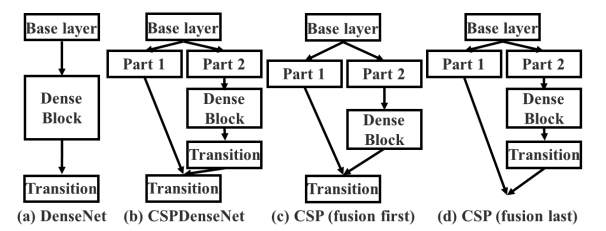
\includegraphics[scale=0.6]{images/csp_block.png}
\caption{CSP模块}
\label{Fig.csp}
\end{figure}

\subsection{Loss}


\subsection{Inference}
在yolov5的推理部分中,预测pred的通道为xywh,obj\_conf, nc。首先,使用conf\_thres 对 obj\_conf 进行过滤,保留一定数目的bbox,然后对所有的类别概率进行重计算$nc\_conf = obj\_conf * nc\_conf$,

\section{backbone}
\subsection{Regularization}
\subsubsection{Dropout}
原理,dropout随机丢弃神经元(全连接中输入神经元),实现方式为$keep_prob$,每个神经元生成一个随机数$k,k<keep_prob$即丢弃。优点,该方法有利于分类中泛化能力的提升.
\subsubsection{Drop Connect}
\subsubsection{Drop block}


\section{Refinedet}
\subsection{Anchor}
Refine中的anchor计算。对于每一个feature map, 首先计算其mesh grid,然后计算每个框的中心点$(x,y)=(\frac{i+0.5}{feat\_size},\frac{j+0.5}{feat\_size})$,然后根据每个feature map对应的anchor box的大小,计算anchor的长和宽$WH_{ki}=\frac{box_k}{image\_size}$, k表示第k层特征图,i表示第i个网格. e.g, 使用四个feature level, $box=[32,64,128,256], image\_size=320, feat\_size=[40,20,10,5], aspect\_ ratio=[2,2,2,2]$, 那么最终生成$40*40*3+20*20*3+10*10*3+5*5*3=6375$个anchor.

\subsection{Loss}
计算过程分为arm和odm,其中arm预测分别输出$num\_anchor*4$和$num\_anchor*2$通道的特征图(坐标,是否包含目标);odm预测分别输出$num\_anchor*4$和$num\_anchor*num\_classes$通道的特征图(坐标,类别数量)。每层特征图的目标数量则为$N_i*H_i*num\_anchor$。

在loss计算过程中,分别计算分类loss和回归loss.其中分类使用交叉熵,回归使用smooth l1



\section{Dataset}
\subsection{COCO Dataset}
COCO dataset 全称 Common Objects in Context. 共有80个类。共有三种标注类型:object instance, object keypoints, image captions。使用json文件进行存储。
\subsubsection{object instance}
{
    "info": info,
    "licenses": [license],
    "images": [image],
    "annotations": [annotation],
    "categories": [category]
}

\section{Detector}
\subsection{CornerNet, CenterNet}
\subsubsection{targets computation}
在anchor free网络中,生成gt bbox的heatmap target时,相应的高斯半径的计算方式如下。一共存在三种情况:
1,生成的target与gt bbox有重叠部分,其中一个corner在gt box内部,另一个在gt box外部。
\begin{gather}
        \cfrac{(w-r)*(h-r)}{w*h+(w+h)r-r^2} \ge {iou} \quad\Rightarrow\quad
        {r^2-(w+h)r+\cfrac{1-iou}{1+iou}*w*h} \ge 0 \\
        {a} = 1,\quad{b} = {-(w+h)},\quad{c} = {\cfrac{1-iou}{1+iou}*w*h} \\
        {r} \le \cfrac{-b-\sqrt{b^2-4*a*c}}{2*a}
\end{gather}
2.两个corner都在gt box里面
\begin{gather}
\cfrac{(w-2*r)*(h-2*r)}{w*h} \ge {iou} \quad\Rightarrow\quad
        {4r^2-2(w+h)r+(1-iou)*w*h} \ge 0 \\
        {a} = 4,\quad {b} = {-2(w+h)},\quad {c} = {(1-iou)*w*h} \\
        {r} \le \cfrac{-b-\sqrt{b^2-4*a*c}}{2*a}
\end{gather}
3.两个corner都在gt box外部
\begin{gather}
\cfrac{w*h}{(w+2*r)*(h+2*r)} \ge {iou} \quad\Rightarrow\quad
        {4*iou*r^2+2*iou*(w+h)r+(iou-1)*w*h} \le 0 \\
        {a} = {4*iou},\quad {b} = {2*iou*(w+h)},\quad {c} = {(iou-1)*w*h} \\
        {r} \le \cfrac{-b+\sqrt{b^2-4*a*c}}{2*a}
\end{gather}
高斯核的计算
\begin{align}
\exp^{\cfrac{-(x*x+y*y)}{2*\sigma*\sigma}}
\end{align}

\subsubsection{decode heatmap}
对heatmap进行解码,遵循如下顺序:1. nms on heatmap. 2. get topk positions from heatmap. 3. decode offset and wh size.

\section{Optical Character Recognition}
\subsection{DBNet}
Real-Time Scene Text Detection with Differentiable Binarization\cite{liao2020real}.
\subsubsection{Related work}
最近的OCR可分为两种:Regression-based and segmentation-based.

\textbf{Regression-based methods} 直接回归文本实例的坐标框,使用NMS后处理。大部分模型达不到精准的文本框检测(非矩形,非旋转矩形等),尤其是弯曲的文本位置。

\textbf{Segmentation-based methods} 结合Pixel-level prediction and post-processing 来获取文本位置。
\begin{figure}[htp!]
\centering
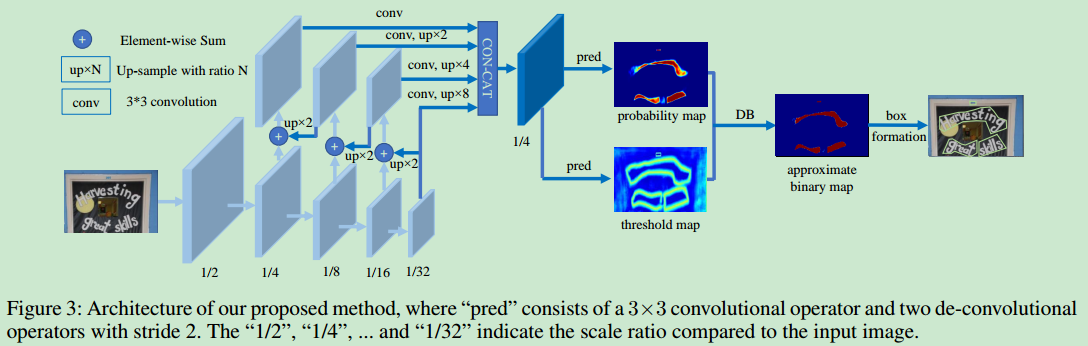
\includegraphics[scale=0.4]{images/dbnet.png}
\caption{Architecture of the DB-Net}
\label{Fig.dbnet}
\end{figure}

\subsubsection{Methodology}
如图Fig. \ref{Fig.dbnet}所示,使用FPN作为backbone,在1/4阶段做预测,生成概率图($P$)和阈值图($T$),并通过P和T来计算approximate binary map($\hat{B}$).二值化过程可表述为如下公式:
\begin{equation}
B_{i,j} = \left\{
\begin{array}{lr}
1 & if \: P_{i,j} >=t, \\
0 & otherwise.
\end{array}
\right.
\label{Eq.binarization}
\end{equation}
\textbf{Differentiable binarization} 公式\ref{Eq.binarization}不可微。所以在训练时不能通过网络对其进行优化,因此论文提出如下近似step function:
\begin{align}
\hat{B}_{i,j}=\dfrac{1}{1+e^{-k(P_{i,j}-T_{i,j})}}
\end{align}
其中,$k$表示增强因子,设置成50.DB提升性能可归结于梯度方向传播。以二值交叉熵为例,定义$f(x)=\dfrac{1}{1+e^{-kx}}$为DB函数,其中$x=P_{i,j}-T_{i,j}$,正类标签的loss $l_+$和负类标签的loss $l_-$分别为:
\begin{equation}
\begin{aligned}
l_+ = -\log{\dfrac{1}{1+e^{-kx}}} \\
l_- = -\log{(1-\dfrac{1}{1+e^{-kx}})}
\end{aligned}
\end{equation}
使用链式规则可以得到如下微分:
\begin{align}
\dfrac{\partial l_+}{\partial x} = -kf(x)e^{-kx} \\
\dfrac{\partial l_x}{\partial x} = kf(x)
\end{align}

\textbf{Label Generation}
PSENet生成方法:给定文本图像,每个文本区域的多边形由一系列线段进行描述:
\begin{align}
G = \{ S_k \}_{k=1}^n
\end{align}
其中,$n$表示顶点数量,在不同的数据集中不一样。ICDAR 2015为4,CTW1500为16.然后使用Vatti clipping算法将多边形$G$收缩程$G_s$得到正类区域.其中,收缩的偏移量D由原多边形的周长L和面积A计算得到:
\begin{align}
D=\dfrac{A(1-r^2)}{L}
\end{align}
$r$为收缩比例,一般设置为0.4. 通过类似方法,为阈值图生成标签。1. 多边形$G$通过相同的偏移$D$进行膨胀得到$G_d$.2. 将$G_s$和$G_d$之间的间隙(gap)作为文本区域的边界,其中阈值图的标签通过计算距离$G$中最近的线段距离得到。

\textbf{Optimization}

Loss表示为概率图$L_s$, 二值图$ L_b $和阈值图$L_t$的加权和:
\begin{align}
L=L_s + \alpha \times L_b + \beta \times L_t
\end{align}
$\alpha$和$\beta$分别设置为1.0和10。对$L_s$和$L_b$应用binary cross-entropy(BCE)loss,使用hard negative mining来缓解正负样本的非平衡问题:
\begin{align}
L_s = L_b = \sum_{i \in S_l}{y_i \log{x_i} + (1 - y_i) \log{1 - x_i}} 
\end{align}
其中,$S_l$为采样集,正负样本比例为1:3.

$L_t$使用$L_1$距离和来计算loss,为膨胀后的文本多边形区域$G_d$内预测和标签的距离:
\begin{align}
L_t = \sum_{i \in R_d}{\left| y_i^* - x_i^* \right|}
\end{align}
其中,$R_d$为膨胀后的多边形$G_d$内的像素索引集合,$y_i^*$为阈值图标签

在推理阶段,可以只用概率图或近似二值图来生成文本坐标框,其结果相似,任选一即可。论文中,为了更好的效率,使用概率图来生成文本框,这样可以移除阈值图。即,box处理过程为三个步骤:1)从概率图/近似二值图通过固定阈值(0.2)来首次二值化得到二值化图; 2)从二值图得到连接区域(收缩的文本区域); 3)使用偏移量$D'$, Vatti clipping算法来膨胀收缩区域。$D'$计算方式为:
\begin{align}
D' = \dfrac{A' \times r'}{L'}
\end{align}
其中,$A'$为收缩多边形的面积;$L'$为收缩多边形的周长;$r'$通过经验设置为$1.5$.

\subsubsection{Implementation Details}
数据集介绍: \textbf{SynthText},\textbf{MLT-2017 dataset},\textbf{ICDAR 2015 dataset},\textbf{MSRA-TD500 dataset},\textbf{CTW1500 dataset},\textbf{Total-Text dataset}.

训练时,使用SynthText预训练100k iteration, 然后在真实样本上微调1200epochs。batch size 16,使用余弦学习率下降策略。其中当前迭代的学习率为$lr_{init} \times (1 - \dfrac{iter}{max\_iter})^{power}$.初始学习率为$0.007$,$power$为0.9.weight decay of 0.0001, momentum of 0.9.

数据增强:1)随机旋转,角度区间$(-10^\circ,10^\circ)$;2)随机裁剪;3)随机翻转。所有处理图片均resize到640x640。

\bibliographystyle{IEEEtran}
\bibliography{reference.bib}


\end{document}